\documentclass[]{article}
\usepackage{lmodern}
\usepackage{amssymb,amsmath}
\usepackage{ifxetex,ifluatex}
\usepackage{fixltx2e} % provides \textsubscript
\ifnum 0\ifxetex 1\fi\ifluatex 1\fi=0 % if pdftex
  \usepackage[T1]{fontenc}
  \usepackage[utf8]{inputenc}
\else % if luatex or xelatex
  \ifxetex
    \usepackage{mathspec}
  \else
    \usepackage{fontspec}
  \fi
  \defaultfontfeatures{Ligatures=TeX,Scale=MatchLowercase}
\fi
% use upquote if available, for straight quotes in verbatim environments
\IfFileExists{upquote.sty}{\usepackage{upquote}}{}
% use microtype if available
\IfFileExists{microtype.sty}{%
\usepackage{microtype}
\UseMicrotypeSet[protrusion]{basicmath} % disable protrusion for tt fonts
}{}
\usepackage[margin=1in]{geometry}
\usepackage{hyperref}
\hypersetup{unicode=true,
            pdftitle={Erik's Covid-19 Chart Pack},
            pdfborder={0 0 0},
            breaklinks=true}
\urlstyle{same}  % don't use monospace font for urls
\usepackage{graphicx,grffile}
\makeatletter
\def\maxwidth{\ifdim\Gin@nat@width>\linewidth\linewidth\else\Gin@nat@width\fi}
\def\maxheight{\ifdim\Gin@nat@height>\textheight\textheight\else\Gin@nat@height\fi}
\makeatother
% Scale images if necessary, so that they will not overflow the page
% margins by default, and it is still possible to overwrite the defaults
% using explicit options in \includegraphics[width, height, ...]{}
\setkeys{Gin}{width=\maxwidth,height=\maxheight,keepaspectratio}
\IfFileExists{parskip.sty}{%
\usepackage{parskip}
}{% else
\setlength{\parindent}{0pt}
\setlength{\parskip}{6pt plus 2pt minus 1pt}
}
\setlength{\emergencystretch}{3em}  % prevent overfull lines
\providecommand{\tightlist}{%
  \setlength{\itemsep}{0pt}\setlength{\parskip}{0pt}}
\setcounter{secnumdepth}{0}
% Redefines (sub)paragraphs to behave more like sections
\ifx\paragraph\undefined\else
\let\oldparagraph\paragraph
\renewcommand{\paragraph}[1]{\oldparagraph{#1}\mbox{}}
\fi
\ifx\subparagraph\undefined\else
\let\oldsubparagraph\subparagraph
\renewcommand{\subparagraph}[1]{\oldsubparagraph{#1}\mbox{}}
\fi

%%% Use protect on footnotes to avoid problems with footnotes in titles
\let\rmarkdownfootnote\footnote%
\def\footnote{\protect\rmarkdownfootnote}

%%% Change title format to be more compact
\usepackage{titling}

% Create subtitle command for use in maketitle
\providecommand{\subtitle}[1]{
  \posttitle{
    \begin{center}\large#1\end{center}
    }
}

\setlength{\droptitle}{-2em}

  \title{Erik's Covid-19 Chart Pack}
    \pretitle{\vspace{\droptitle}\centering\huge}
  \posttitle{\par}
    \author{}
    \preauthor{}\postauthor{}
    \date{}
    \predate{}\postdate{}
  
\usepackage{booktabs}
\usepackage{longtable}
\usepackage{array}
\usepackage{multirow}
\usepackage{wrapfig}
\usepackage{float}
\usepackage{colortbl}
\usepackage{pdflscape}
\usepackage{tabu}
\usepackage{threeparttable}
\usepackage{threeparttablex}
\usepackage[normalem]{ulem}
\usepackage{makecell}
\usepackage{xcolor}

\begin{document}
\maketitle

Data updated 2020-06-26 19:11:38. World data are from
\href{https://github.com/NovelCovid/API}{Worldometers}. National and
state-level mortality, case, and testing data are from
\href{https://covidtracking.com}{Johns-Hopkins University}. County and
city-level mortality and case data are from the
\href{https://github.com/NovelCovid/API}{New York Times}. Most data
presented in this report were accessed through APIs provided by
\href{https://covidtracking.com}{The COVID Tracking Project} and
\href{https://github.com/NovelCovid/API}{NovelCOVID API}.

\hypertarget{world-data}{%
\section{World Data}\label{world-data}}

There have been 9,703,330 confirmed Covid-19 cases and 490,989 deaths
worldwide.

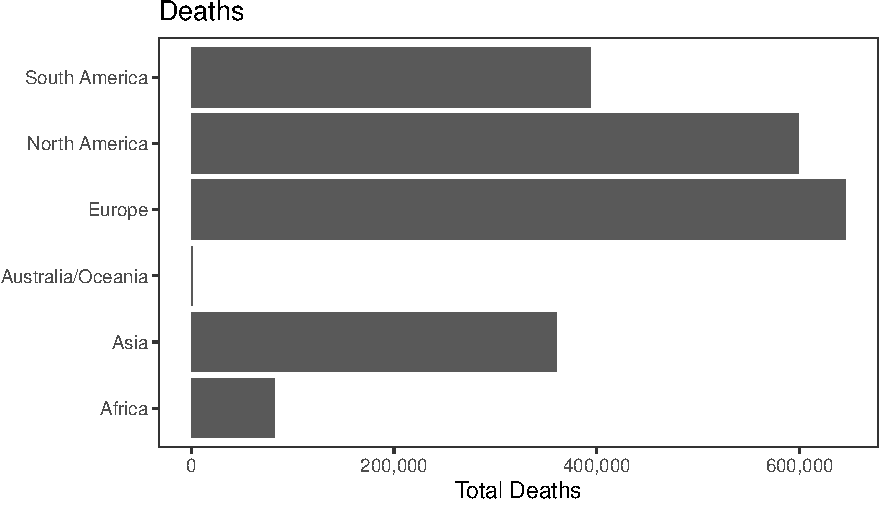
\includegraphics{covid_files/figure-latex/unnamed-chunk-1-1.pdf}

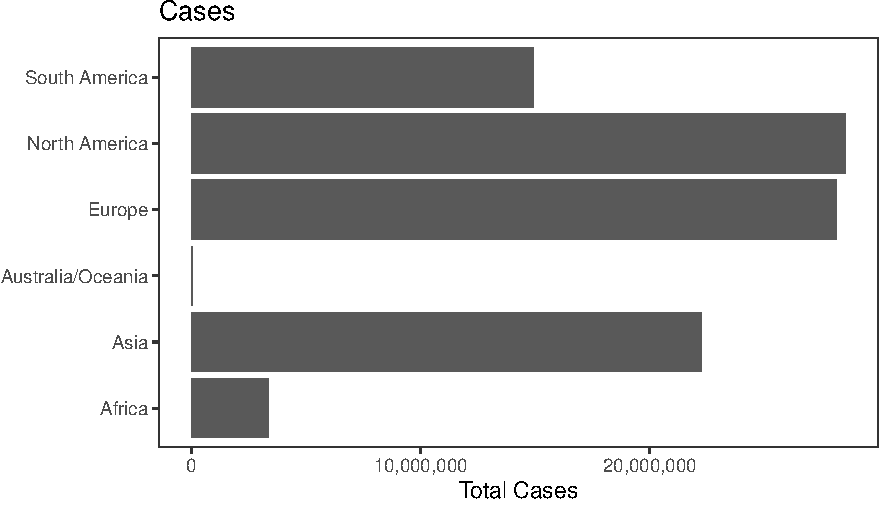
\includegraphics{covid_files/figure-latex/unnamed-chunk-2-1.pdf}

\newpage

\begin{table}[!h]

\caption{\label{tab:unnamed-chunk-3}Top Countries by Total Cases}
\centering
\begin{tabular}{l|r|r|r|r}
\hline
Country & Cases & Deaths & New Cases & New Deaths\\
\hline
USA & 2,504,588 & 126,780 & 40,184 & 649\\
\hline
Brazil & 1,233,147 & 55,054 & 40,673 & 1,180\\
\hline
Russia & 613,994 & 8,605 & 7,113 & 92\\
\hline
India & 491,170 & 15,308 & 18,185 & 401\\
\hline
UK & 307,980 & 43,230 & 1,118 & 149\\
\hline
Spain & 294,566 & 28,330 & 400 & 3\\
\hline
Peru & 268,602 & 8,761 & 3,913 & 175\\
\hline
Chile & 259,064 & 4,903 & 4,648 & 172\\
\hline
Italy & 239,706 & 34,678 & 296 & 34\\
\hline
Iran & 215,096 & 10,130 & 2,595 & 134\\
\hline
Mexico & 196,847 & 24,324 & 5,437 & 947\\
\hline
Germany & 193,785 & 9,012 & 531 & 9\\
\hline
Turkey & 193,115 & 5,046 & 1,458 & 21\\
\hline
Pakistan & 192,970 & 3,903 & 4,044 & 148\\
\hline
Saudi Arabia & 170,639 & 1,428 & 3,372 & 41\\
\hline
France & 161,348 & 29,752 & 0 & 21\\
\hline
Bangladesh & 126,606 & 1,621 & 3,946 & 39\\
\hline
South Africa & 118,375 & 2,292 & 6,579 & 87\\
\hline
Canada & 102,622 & 8,504 & 380 & 20\\
\hline
Qatar & 91,838 & 106 & 1,060 & 2\\
\hline
\end{tabular}
\end{table}

\newpage

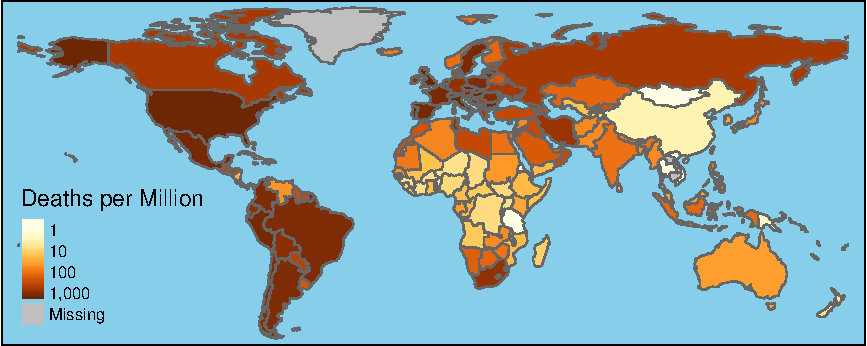
\includegraphics{covid_files/figure-latex/unnamed-chunk-4-1.pdf}

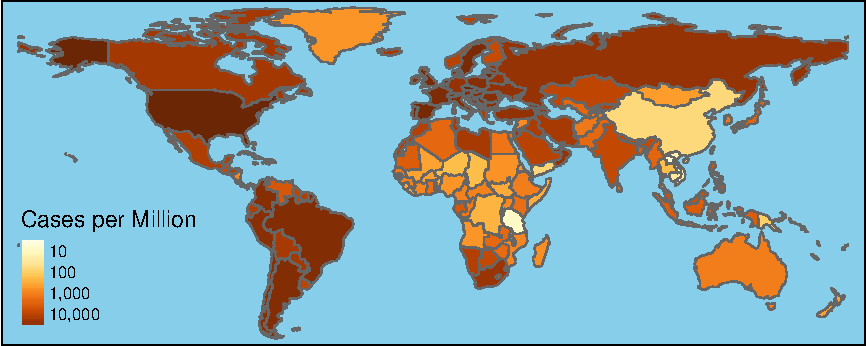
\includegraphics{covid_files/figure-latex/unnamed-chunk-5-1.pdf}

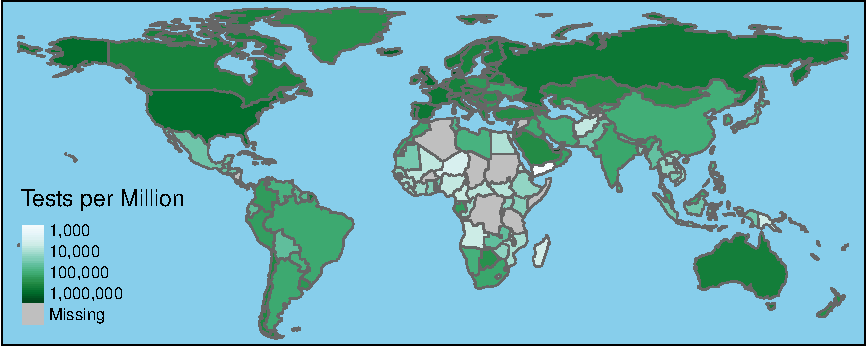
\includegraphics{covid_files/figure-latex/unnamed-chunk-6-1.pdf}

\newpage

\hypertarget{national-data}{%
\section{National Data}\label{national-data}}

There have been 2,455,351 confirmed Covid-19 cases and 118,650 deaths in
the United States.

\begin{table}[!h]

\caption{\label{tab:unnamed-chunk-8}U.S. Deaths and Cases over the Last Two Weeks}
\centering
\begin{tabular}{l|r|r|r|r}
\hline
Date & Cases & Deaths & New Cases & New Deaths\\
\hline
2020-06-26 & 2,455,351 & 118,650 & 44,373 & 619\\
\hline
2020-06-25 & 2,410,978 & 118,031 & 39,061 & 2,500\\
\hline
2020-06-24 & 2,371,917 & 115,531 & 38,706 & 722\\
\hline
2020-06-23 & 2,333,211 & 114,809 & 33,018 & 703\\
\hline
2020-06-22 & 2,300,193 & 114,106 & 27,050 & 282\\
\hline
2020-06-21 & 2,273,143 & 113,824 & 27,287 & 297\\
\hline
2020-06-20 & 2,245,856 & 113,527 & 31,958 & 621\\
\hline
2020-06-19 & 2,213,898 & 112,906 & 31,055 & 647\\
\hline
2020-06-18 & 2,182,843 & 112,259 & 27,512 & 693\\
\hline
2020-06-17 & 2,155,331 & 111,566 & 23,871 & 778\\
\hline
2020-06-16 & 2,131,460 & 110,788 & 23,638 & 713\\
\hline
2020-06-15 & 2,107,822 & 110,075 & 18,655 & 379\\
\hline
2020-06-14 & 2,089,167 & 109,696 & 21,240 & 356\\
\hline
2020-06-13 & 2,067,927 & 109,340 & 25,134 & 693\\
\hline
\end{tabular}
\end{table}

\newpage

\hypertarget{deaths}{%
\subsection{Deaths}\label{deaths}}

Because the effects of the virus can take several weeks to manifest in
patients, deaths are a lagging indicator of contagion, but they may be a
more reliable than case counts, which are a function of both the
prevalence of the disease and the rate of testing. The case mortality
rate is a very crude indicator of lethality because a large numbers of
non-lethal cases are likely never detected. A declining case mortality
rate is indicative of more widespread testing.

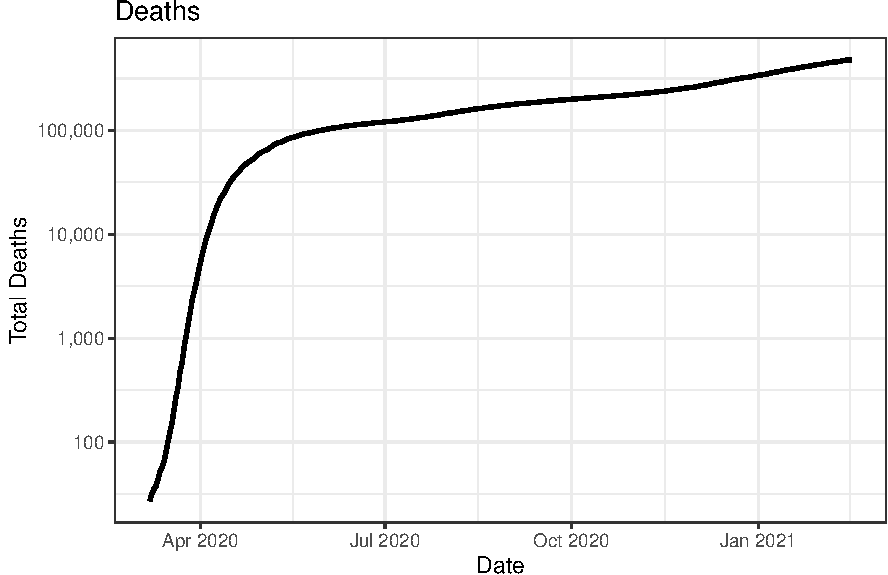
\includegraphics{covid_files/figure-latex/unnamed-chunk-9-1.pdf}

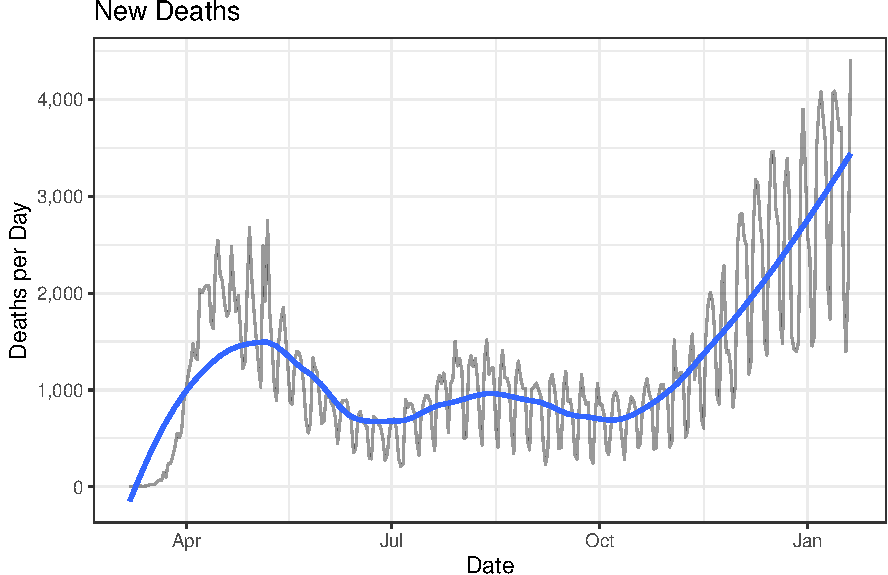
\includegraphics{covid_files/figure-latex/unnamed-chunk-10-1.pdf}

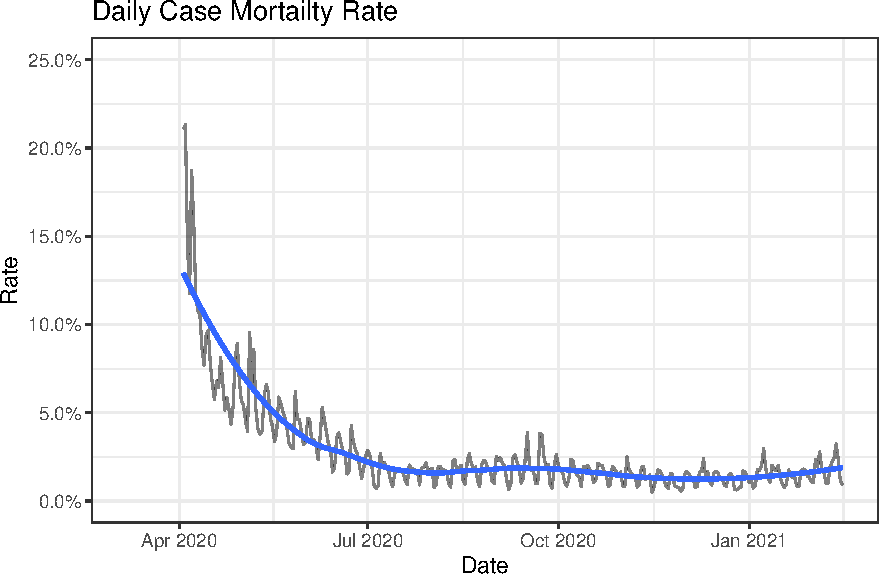
\includegraphics{covid_files/figure-latex/unnamed-chunk-11-1.pdf}

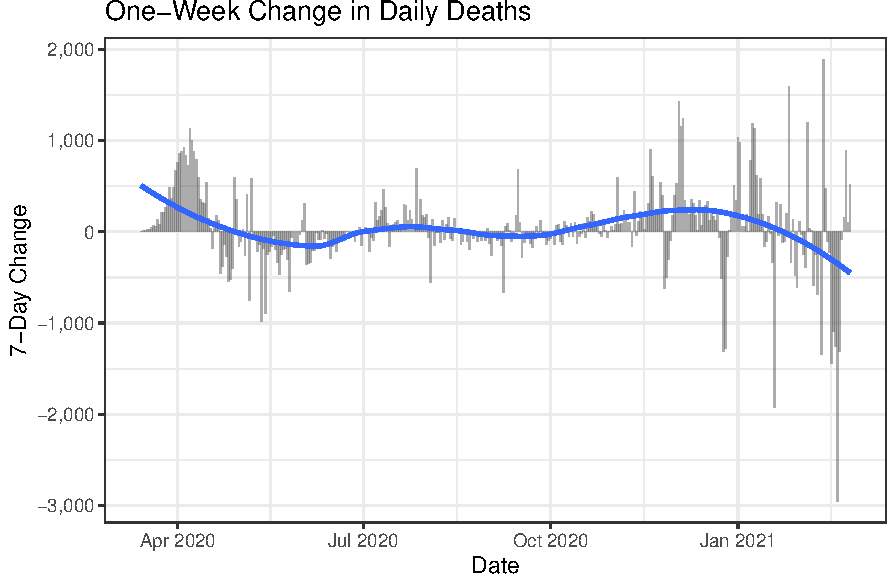
\includegraphics{covid_files/figure-latex/unnamed-chunk-12-1.pdf}

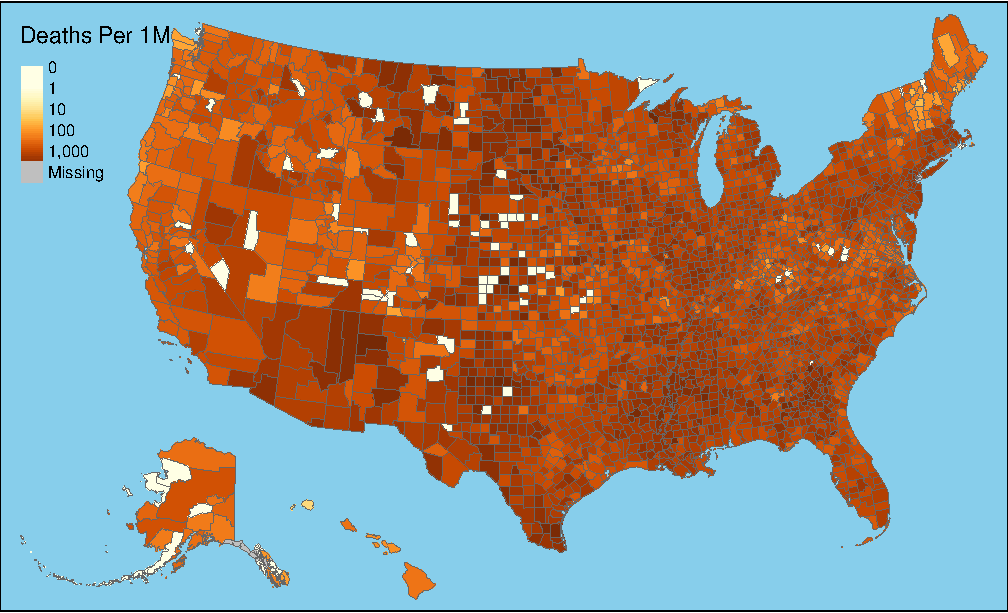
\includegraphics{covid_files/figure-latex/unnamed-chunk-13-1.pdf}

\newpage

\hypertarget{cases}{%
\subsection{Cases}\label{cases}}

Reported cases are a function of both the spread of the disease and the
prevalence of testing.

\includegraphics{covid_files/figure-latex/unnamed-chunk-14-1.pdf}

\includegraphics{covid_files/figure-latex/unnamed-chunk-15-1.pdf}

\includegraphics{covid_files/figure-latex/unnamed-chunk-16-1.pdf}

\includegraphics{covid_files/figure-latex/unnamed-chunk-17-1.pdf}

\newpage

\hypertarget{testing}{%
\subsection{Testing}\label{testing}}

Widespread testing is necessary for managing the spread of the disease.
The following charts show how testing in the United States has changed
over time. When the supply of available tests is limited, they are
typically only used for patients whose symptoms suggest they are likely
to have contracted the virus. A high positive test rate indicates that
testing capacity is constrained.

\includegraphics{covid_files/figure-latex/unnamed-chunk-18-1.pdf}

\includegraphics{covid_files/figure-latex/unnamed-chunk-19-1.pdf}

\includegraphics{covid_files/figure-latex/unnamed-chunk-20-1.pdf}

\includegraphics{covid_files/figure-latex/unnamed-chunk-21-1.pdf}

\newpage

\hypertarget{state-data}{%
\section{State Data}\label{state-data}}

This section summarizes state-level data. Most data are reported for the
largest 15 states by population, which account for NaN percent of the
total U.S. population.

\hypertarget{deaths-1}{%
\subsection{Deaths}\label{deaths-1}}

\includegraphics{covid_files/figure-latex/unnamed-chunk-24-1.pdf}

\includegraphics{covid_files/figure-latex/unnamed-chunk-25-1.pdf}

\includegraphics{covid_files/figure-latex/unnamed-chunk-26-1.pdf}
\newpage

\includegraphics{covid_files/figure-latex/unnamed-chunk-27-1.pdf}

\includegraphics{covid_files/figure-latex/unnamed-chunk-28-1.pdf}

\newpage

\hypertarget{cases-1}{%
\subsection{Cases}\label{cases-1}}

\includegraphics{covid_files/figure-latex/unnamed-chunk-30-1.pdf}

\includegraphics{covid_files/figure-latex/unnamed-chunk-31-1.pdf}

\includegraphics{covid_files/figure-latex/unnamed-chunk-32-1.pdf}
\newpage

\includegraphics{covid_files/figure-latex/unnamed-chunk-33-1.pdf}

\includegraphics{covid_files/figure-latex/unnamed-chunk-34-1.pdf}

\newpage

\hypertarget{testing-1}{%
\subsection{Testing}\label{testing-1}}

\includegraphics{covid_files/figure-latex/unnamed-chunk-35-1.pdf}

\includegraphics{covid_files/figure-latex/unnamed-chunk-36-1.pdf}

\newpage

\includegraphics{covid_files/figure-latex/unnamed-chunk-37-1.pdf}

\includegraphics{covid_files/figure-latex/unnamed-chunk-38-1.pdf}
\newpage

Interpretation of differences in case rates across states is complicated
by the fact that those states that do more thorough testing will
invariably uncover more cases. A lower positive test rate is an
indication that a state is doing more comprehensive testing since, when
testing is rationed, only those individuals who are more likely to test
positive are typically tested. The following chart compares the one-week
increase in detected cases to the the number of tests administered by
each state relative to population. The states of greatest current
concern are those with both a large increase in detected cases and a
relatively small increase in tests. These states lie in the upper-left
of the chart.

\includegraphics{covid_files/figure-latex/unnamed-chunk-39-1.pdf}

\newpage

\hypertarget{local-data}{%
\section{Local Data}\label{local-data}}

The following charts and tables present mortality, case, and testing
data for the Washington DC metropolitan area and adjacent states.

\begin{table}[!h]

\caption{\label{tab:unnamed-chunk-42}Latest Local Data}
\centering
\begin{tabular}{l|r|r|r|r}
\hline
State & Cases & Deaths & New Cases & New Deaths\\
\hline
DC & 10,185 & 546 & 26 & 3\\
\hline
MD & 66,115 & 3,142 & 338 & 13\\
\hline
VA & 60,570 & 1,700 & 624 & 25\\
\hline
\end{tabular}
\end{table}

\newpage

\hypertarget{deaths-2}{%
\subsection{Deaths}\label{deaths-2}}

\includegraphics{covid_files/figure-latex/unnamed-chunk-43-1.pdf}

\includegraphics{covid_files/figure-latex/unnamed-chunk-44-1.pdf}

\includegraphics{covid_files/figure-latex/unnamed-chunk-45-1.pdf}

\includegraphics{covid_files/figure-latex/unnamed-chunk-46-1.pdf}

\includegraphics{covid_files/figure-latex/unnamed-chunk-47-1.pdf}

\newpage

\hypertarget{cases-2}{%
\subsection{Cases}\label{cases-2}}

\includegraphics{covid_files/figure-latex/unnamed-chunk-48-1.pdf}

\includegraphics{covid_files/figure-latex/unnamed-chunk-49-1.pdf}

\includegraphics{covid_files/figure-latex/unnamed-chunk-50-1.pdf}

\includegraphics{covid_files/figure-latex/unnamed-chunk-51-1.pdf}

\includegraphics{covid_files/figure-latex/unnamed-chunk-52-1.pdf}

\newpage

\hypertarget{testing-2}{%
\subsection{Testing}\label{testing-2}}

\includegraphics{covid_files/figure-latex/unnamed-chunk-53-1.pdf}

\includegraphics{covid_files/figure-latex/unnamed-chunk-54-1.pdf}

\includegraphics{covid_files/figure-latex/unnamed-chunk-55-1.pdf}


\end{document}
